\documentclass[aps,prb,onecolumn,notitlepage,showpacs,floatfix,superscriptaddress]{revtex4-1}
\usepackage{dcolumn}
\usepackage{tabularx}
\usepackage{bm}
\usepackage{soul}
\usepackage{amsmath,amssymb,graphicx}
\usepackage[colorlinks=true,citecolor=blue,urlcolor=blue,linkcolor=blue]{hyperref}
\usepackage{environ}
\usepackage{relsize}
\NewEnviron{eqnsplit}{%
\begin{equation}
\begin{split}
  \BODY
\end{split}
\end{equation}
}

\newcommand{\mrm}[1]{\mathrm{#1}}
\newcommand{\ang}{\mathrm{\AA}}

\bibliographystyle{apsrev4-1}

%%%%%%%%%%%%%%%%%%%%%%%%%%%%%%%%%%%%%%%%%%%%%%%%
\begin{document}

\title{Band Gap Renormalization - Plasmon Pole Approximation}

\author{Avinash Rustagi}
\email{arustag@ncsu.edu}
\affiliation{Department of Physics, North Carolina State University, Raleigh, NC 27695}
%
\date{\today}
%%%%%%%%%%%%%%%%%%%%%%%%%%%%%%%%%%%%%%%%%%%%%%%%
\begin{abstract}
The objective is to evaluate the Band Gap Renormalization (BGR) using the single plasmon pole approximation (SPPA) for the dielectric constant. 
\end{abstract}
\maketitle
BGR can be simply estimated through the change in energy dispersion due to interaction i.e. Self energy. Considering the screened interaction $W(q,iq_n)$ (in Matsubara formalism), we can simply compute the self energy using the $G_0 W$ approximation.
\begin{figure}[hbtp]
\centering
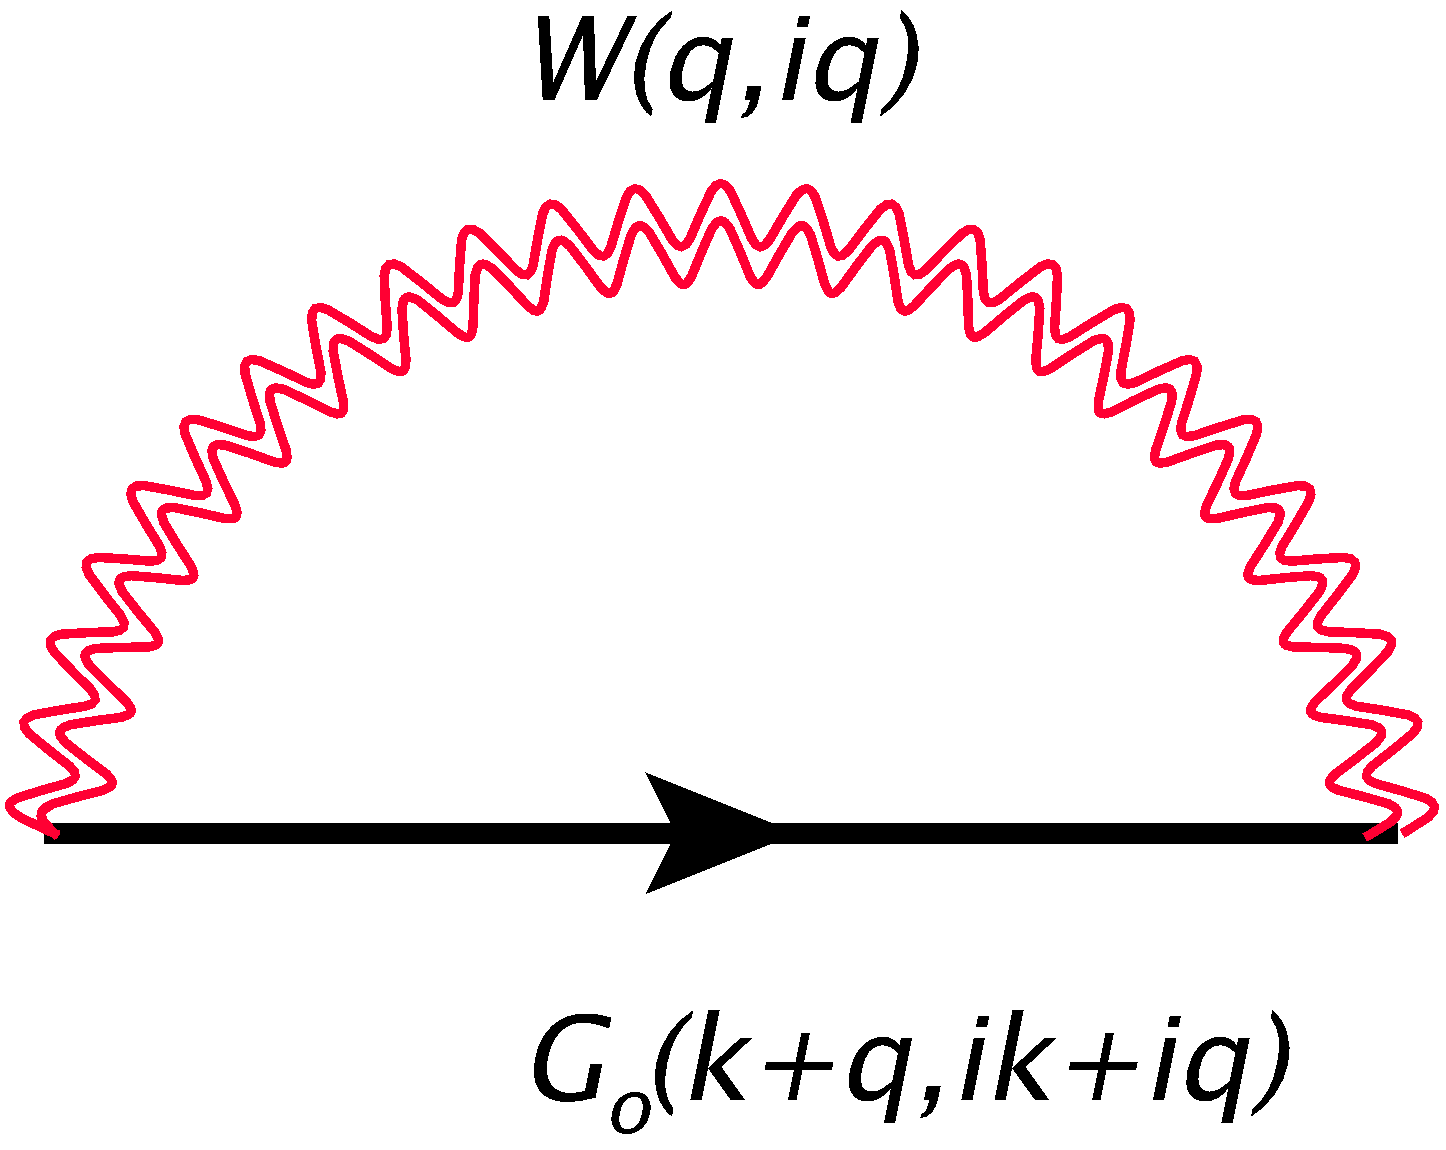
\includegraphics[scale=0.1]{G0W.png}
\caption{Self Energy Diagram}
\end{figure}
\begin{equation}
\Sigma(k,ik_n) = -\dfrac{1}{\beta} \sum_{q,iq_n} W(q,iq_n) G_0 (k+q,ik_n+iq_n)
\end{equation}
where the non-interacting Green function
\begin{equation}
 G_0 (k+q,ik_n+iq_n) = \dfrac{1}{ik_n + iq_n -\varepsilon_{k+q}}
\end{equation}
and the screened interaction $W(q,iq_n)$ is
\begin{equation}
W(q,iq_n) = \dfrac{V(q)}{\varepsilon(q,iq_n)} = V(q) + V(q) \left[ \dfrac{1}{\varepsilon(q,iq_n)}-1\right]
\end{equation}
The plasmon-pole approximation is used to construct the full dielectric function $\varepsilon(q,iq_n)$ which replaces the continuum of poles in the Lindhard function by one effective plasmon-pole $\omega_q$. Therefore
\begin{equation}
\begin{split}
\dfrac{1}{\varepsilon(q,iq_n)}&=1+ \dfrac{\omega_p^2}{( iq_n)^2-\omega_q^2}
\end{split} 
\end{equation}
Therefore
\begin{equation}
\begin{split}
\Sigma(k,ik_n) &= -\dfrac{1}{\beta} \sum_{q,iq_n} \left[ V(q) + V(q) \left[ \dfrac{1}{\varepsilon(q,iq_n)}-1\right] \right] G_0 (k+q,ik_n+iq_n) \\
&=  -\dfrac{1}{\beta} \sum_{q,iq_n}V(q)  G_0 (k+q,ik_n+iq_n) -\dfrac{1}{\beta} \sum_{q,iq_n} V(q) \left[ \dfrac{1}{\varepsilon(q,iq_n)}-1\right] G_0 (k+q,ik_n+iq_n) \\
&=\Sigma_x(k,ik_n) +\Sigma_c(k,ik_n) 
\end{split}
\end{equation}
where the exchange and correlation self energy terms can be evaluated.
\begin{equation}
\Sigma_x(k,ik_n) = -\dfrac{1}{\beta} \sum_{q,iq_n}V(q)  G_0 (k+q,ik_n+iq_n) = -\sum_q V(q) f_{k+q}
\end{equation}
where $f_{k+q}$ is the Fermi-Dirac distribution function,
\begin{equation}
\begin{split}
\Sigma_c(k,ik_n) &= -\dfrac{1}{\beta} \sum_{q,iq_n}V(q) \left[ \dfrac{1}{\varepsilon(q,iq_n)}-1\right] G_0 (k+q,ik_n+iq_n)  \\
&= -\dfrac{1}{\beta} \sum_{q,iq_n}V(q) \dfrac{\omega_p^2}{( iq_n)^2-\omega_q^2} G_0 (k+q,ik_n+iq_n)  \\
&= \sum_q V(q) \dfrac{\omega_p^2}{2\omega_q} \left[\dfrac{f_{k+q}+g_q}{ik_n - \varepsilon_{k+q}+\omega_q}+\dfrac{1-f_{k+q}+g_q}{ik_n - \varepsilon_{k+q}-\omega_q} \right]
\end{split}
\end{equation}
and $g_q = 1/(\exp(\omega_q /T)-1)$. Thus the renormalization of band edge due to carriers can be evaluated by analytic continuation of the self energy and setting momenta to the band extrema location:  $\omega = \varepsilon_k$ and $k=0$ here.
\begin{equation}
\Delta E = \Sigma(k,\varepsilon_k)\vert_{k=0}
\end{equation}
This is also refereed to as the rigid band shift.

\section*{BGR in 2D Electron-Hole System}
In 2D, considering an electron hole plasma with a reduced mass $m$: $m^{-1}=m_e^{-1}+m_h^{-1}$, the electrons cause shift in the CB minima and the holes cause shift of the VB maxima. Thus the BGR will have contribution from both the species of charge carriers
\begin{equation}
\begin{split}
\Delta E_G &= \Sigma_e(k,\varepsilon_k)\vert_{k=0}+\Sigma_h(k,\varepsilon_k)\vert_{k=0} \\
&= -\sum_{q,i=\{e,h\} }V(q) f_{i,q} + \sum_{q,i=\{e,h\} } V(q) \dfrac{\omega_p^2}{2\omega_q} \left[\dfrac{f_{i,q}+g_q}{\varepsilon_{i,0} - \varepsilon_{i,q}+\omega_q}+\dfrac{1-f_{i,q}+g_q}{\varepsilon_{i,0} - \varepsilon_{i,q}-\omega_q} \right]
\end{split}
\end{equation}
In accordance with Schmitt-Rink et. al [Solid State Communications, Vol.52, No.2, pp.123-125, 1984], we express all lengths and energies in units of exciton Bohr radius and Rydberg.
\begin{equation}
a_0 = \dfrac{\varepsilon_0}{2 m e^2} \qquad E_0 = \dfrac{1}{2ma_0^2} = \dfrac{e^2}{\varepsilon_0 a_0}
\end{equation}
Therefore
\begin{itemize}
\item Interaction potential $V(q)=\dfrac{2\pi e^2}{\varepsilon_0 q} = \dfrac{2\pi a_o^2}{qa_0} E_0$
\item Plasma Frequency $\omega_p^2 = \dfrac{2\pi n e^2 q}{\varepsilon_0 m} = 4\pi (na_0^2) (qa_0) E_0^2$
\item Energy dispersion $\varepsilon_i = \dfrac{k^2}{2 m_i} = \dfrac{m}{m_i} (ka_0)^2 E_0$ where $i=\{e,h\}$ [Spin Degenerate]
\item Number Density $n=2\sum_k f_{i,k}$ $\Rightarrow$ $na_0^2 = \dfrac{\bar{T}}{2\pi} \dfrac{m_i}{m} \text{Ln} (1+ \exp(\bar{\mu_i}/\bar{T})) $ where $T=\bar{T} E_0$
\item Chemical Potential $\bar{\mu_i} = \bar{T} \, \text{Ln} \left[\exp\left({\dfrac{2\pi n (na_0^2)}{\bar{T}m_i}}\right)-1 \right]$
\item Thomas Fermi Screening wavenumber $\kappa = \dfrac{2\pi e^2}{\varepsilon_0} \mathlarger{\sum_{i}} \dfrac{\partial n}{\partial \mu_i}$ where $\mu_i = \bar{\mu_i} E_0$ is the chemical potential $\Rightarrow$ $\kappa a_0 = 2\pi \left[\dfrac{\partial (na_0^2)}{\partial \bar{\mu_e}}+\dfrac{\partial (na_0^2)}{\partial \bar{\mu_h}} \right] = \dfrac{m_e}{m}\dfrac{1}{1+e^{-\bar{\mu_e}/\bar{T}}}+\dfrac{m_h}{m}\dfrac{1}{1+e^{-\bar{\mu_h}/\bar{T}}}$ .
\item Plasmon Pole with Lundquist correction $\omega_q^2 = \omega_p^2 (1+q/\kappa) + (\varepsilon_{e,q}+\varepsilon_{h,q})^2/4$
\end{itemize}
Thus computing the BGR for Coulomb interaction in 2D 
\begin{figure}[hbtp]
\centering
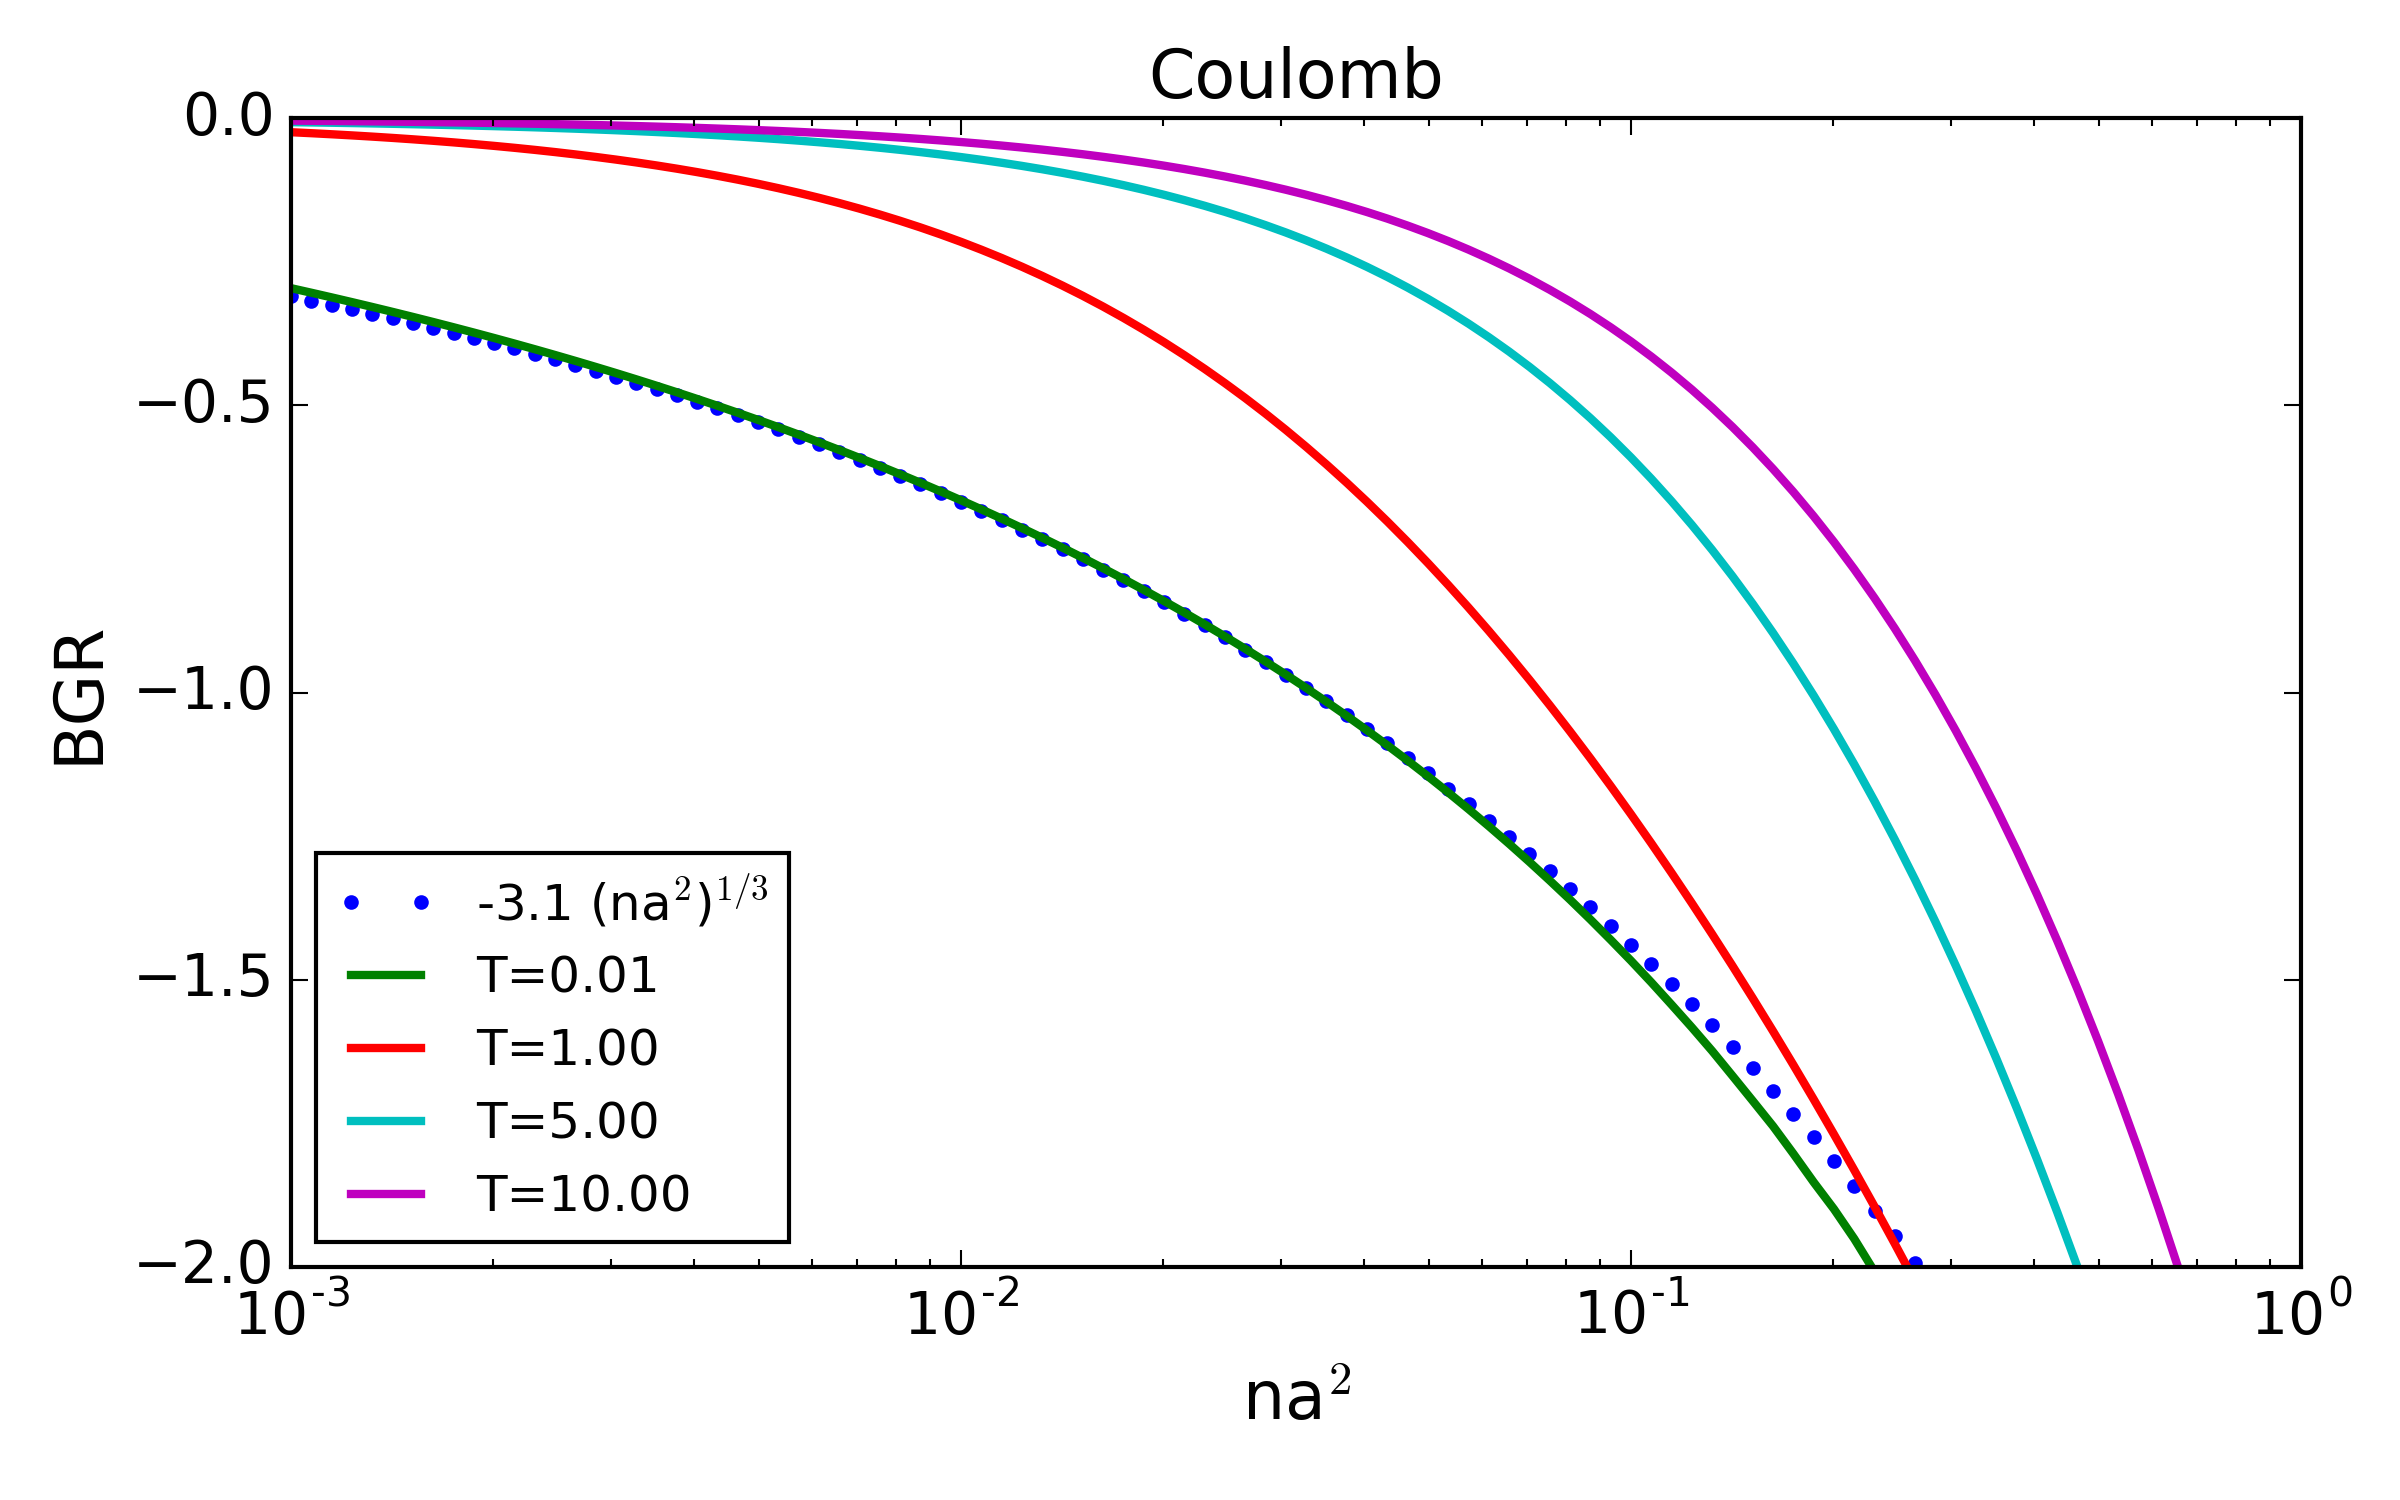
\includegraphics[scale=0.5]{BGR_Haug.png}
\caption{BGR - Coulomb in 2D - in units of $E_0$. Temperatures are in units of $E_0$.}
\end{figure}
where the expression $-3.1 (n a_0^2)^{1/3} E_0$ is a good approximation to BGR for T=0.
\end{document}